\documentclass[xcolor=table]{beamer}
\usepackage{fontspec}
\usepackage{natbib}
\usepackage{gb4e} 
\usepackage[table]{xcolor}
\usepackage{booktabs} 
%\usepackage{color}
\usepackage{graphicx}
\usepackage{tikz}
\usetikzlibrary{trees}
\usepackage{bibentry}

% \setmainfont[Mapping=tex-text]{Charis SIL}
\let\sfdefault\rmdefault
%\newcommand{\racine}[1]{\begin{math}\sqrt{#1}\end{math}} 
\newfontfamily\phon[Mapping=tex-text,Ligatures=Common,Scale=MatchLowercase]{Charis SIL} 
\newcommand{\ipa}[1]{{\phon\textit{#1}}} %API tjs en italique
\newcommand{\grise}[1]{\cellcolor{lightgray}\textbf{#1}} 
\newcommand{\ro}{$\Sigma$} 
 \newcommand{\bleu}[1]{{\color{blue}#1}}
\newcommand{\rouge}[1]{{\color{red}#1}} 
\newcommand{\bordeau}[1]{{\color{purple}#1}} 
\newcommand{\jpg}[2]{\bleu{\ipa{#1}} `#2'}
\newcommand{\jb}[2]{\bordeau{\ipa{#1}} `#2'}
\newcommand{\tib}[2]{\rouge{\ipa{#1}} `#2'}
 \begin{document}



 \title{Two issues in Trans-Himalayan comparative linguistics}
 \author{Guillaume Jacques}
 \maketitle


 \begin{frame} 
 \frametitle{Two issues in Trans-Himalayan comparative linguistics}
 \begin{itemize}[<+->]
 \item Loanwords vs cognates
 \item Morphology and degree of cognacy
 \end{itemize}
\end{frame}

 \begin{frame} 
 \frametitle{Loanwords vs cognates}
 \begin{itemize}[<+->]
 \item Main sources of loanwords: 
  \begin{itemize}[<+->]
  \item Chinese
  \item Tibetan
    \item Indic
   \end{itemize}
 \item Borrowings between closely related languages
 \item In which conditions should borrowings be counted as cognates?
 \end{itemize}
\end{frame}

 \begin{frame} 
 \frametitle{Loanwords from Tibetic languages}
 \begin{itemize}[<+->]
 \item Pervasive in languages of Tibetan-influenced areas:
  \begin{itemize}[<+->]
 \item Gyalrongic (and other languages of Tibetan Sichuan)
   \item languages of Bhutan and of the South Tibet/Arunachal area
  \item West-Himalayish
  \end{itemize}
 \item How to distinguish cognates from loanwords?
 \end{itemize}
\end{frame}

 \begin{frame} 
 \frametitle{\bordeau{Loanwords} from \rouge{Tibetan} into Gyalrongic}
Phonological criteria (Sound changes)
 \begin{enumerate}[<+->]
 \item Words that have \textsc{not} undergone all of the sound changes of the native vocabulary are \bordeau{borrowings} (necessary but not sufficient condition).
 \begin{itemize}[<+->] 
\item  \jb{smɯn}{have a result} borrowing from \tib{smin}{be ripe} vs the cognate \jpg{smi}{be cooked, be ripe}, with loss of final *\ipa{-n})
%\item 
  \end{itemize}
 \item Words that have \textsc{not} undergone Tibetan-specific sound changes are \bleu{cognates}, unless they can be shown to be borrowings from other languages, or if a sound change in Japhug has removed the effect of the Tibetan sound change  (not necessary but sufficient condition).
  \begin{itemize}[<+->] 
\item  \jpg{kɯβde}{four} is cognate to \tib{bʑi}{four}, unlike \jb{aβʑɯrdu}{square}, borrowing from \tib{bʑi.rdo}{four stones} (\ipa{*l} $\rightarrow$ \ipa{ʑ} in Tibetan)
  \end{itemize}
     \item Words that have undergone Tibetan-specific sound changes (including later Amdo-specific ones) are \bordeau{borrowings}, unless  a parallel sound change can be shown to have taken place in Japhug (not necessary but sufficient condition).
  \begin{itemize}[<+->] 
\item  \jb{ɯ-raŋ}{time, period} from the Amdo prononciation of \tib{riŋ}{time}
  \end{itemize}
 \end{enumerate}
\end{frame}

 \begin{frame} 
 \frametitle{\bordeau{Loanwords} from \rouge{Tibetan} into Gyalrongic II}
Phonological criteria (Phonotactics)
 \begin{enumerate}[<+->]
 \item Words with clusters or rhymes only attested in words related to Tibetan are borrowings.
   \begin{itemize}[<+->] 
 \item \jb{βzdɯ}{collect} from the future tense of \tib{bsdu}{collect}
   \end{itemize}
\item Words with clusters without equivalent in Tibetan are cognate, unless they can be shown to have undergone Japhug-internal morphological derivation.
   \begin{itemize}[<+->] 
 \item \jpg{tɯ-ɕnaβ}{snot} is cognate of Tibetan \tib{snabs}{snot}.
   \end{itemize}
   \end{enumerate} 
\end{frame}
 
  \begin{frame} 
 \frametitle{\bordeau{Loanwords} from \rouge{Tibetan} into Gyalrongic III}
Morphological criteria 
 \begin{enumerate}[<+->]
 \item Words that have Tibetan-specific morphology are \bordeau{borrowings}
  \begin{itemize}[<+->] 
\item \jb{fkaβ}{cover} from the past tense of \tib{ɴgebs, bkab}{cover}
  \end{itemize} 
 \item Identical compound words are all borrowings
  \begin{itemize}[<+->] 
\item \jb{mtɕʰɤtkʰo}{chapel} from Tibetan \tib{mtɕʰod.kʰaŋ}{chapel}
  \end{itemize} 
  \end{enumerate}
\end{frame}


  \begin{frame} 
 \frametitle{\bordeau{Loanwords} from \rouge{Tibetan} into Gyalrongic IV}
Semantic criteria 
 \begin{enumerate}[<+->]
 \item Words that have undergone Tibetan-specific semantic changes are \bordeau{borrowings}
  \begin{itemize}[<+->] 
\item \jb{ʑu}{yoghurt} from Tibetan \tib{ʑo}{yoghurt}
  \end{itemize} 
 \item Words that have \textsc{not} undergone Tibetan-specific semantic changes are \bleu{cognates}
  \begin{itemize}[<+->] 
\item \jpg{tɤ-lu}{milk}, cognate of Tibetan \tib{ʑo}{yoghurt} $\leftarrow$\ipa{*lʲo}
  \end{itemize} 
 \item Words phonologically compatible with Tibetan referring to Buddhism/recent technological innovations  are \bordeau{borrowings}
   \begin{itemize}[<+->] 
\item \jb{βdɯt}{demon} from Tibetan \tib{bdud}{Mâra}
  \end{itemize} 
  \end{enumerate}
\end{frame}

  \begin{frame} 
 \frametitle{Loanwords from Tibetan into Gyalrongic}
The same criteria can be generalized to any pair of languages.
\end{frame}

  \begin{frame} 
 \frametitle{Loanwords between closely related languages}
Much trickier, example Thulung \ipa{yalmu} $\rightarrow$ Khaling \ipa{jālnɛ} `hit'
\end{frame}

  \begin{frame} 
 \frametitle{Morphology}
Need for a more refined notion of cognacy (List 2016)
\end{frame}

  \begin{frame} 
 \frametitle{Morphology: verb derivations in Kiranti I}


  \begin{tikzpicture}
  \node (Bi) at (-2,1) {Bi *\ipa{kʰraːp} (vi)};
 \node (Ai) at (-1.5,-1) {A *\ipa{kʰraːp-t} (vt)};
   \node (AiM) at (-4,-4) {A+M *\ipa{kʰraːp(t)-si} (vi)};
  \node (Ci) at (-4.5,-1) {C *\ipa{kʰraːp-s} (vt)};
    
\tikzstyle{peutetre}=[->,dotted,very thick,>=latex]
\tikzstyle{sur}=[->,very thick,>=latex]
\draw[sur] (Bi)--(Ai);
\draw[sur] (Bi)--(Ci);
\draw[sur] (Ai) to[bend left] (AiM);

\end{tikzpicture}
\end{frame}

  \begin{frame} 
 \frametitle{Morphology: verb derivations in Kiranti II}

  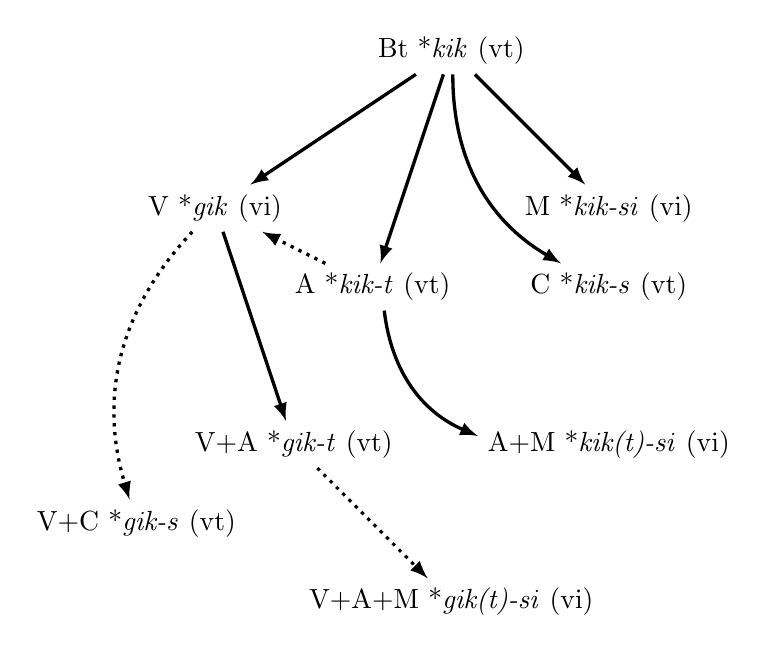
\begin{tikzpicture}
%  \node (Bi) at (-2,1) {Bi *\ipa{kʰraːp} (vi)};
  \node (Bt) at (4,1) {Bt *\ipa{kik} (vt)};
  \node (V) at (1,-1) {V *\ipa{gik} (vi)};
% \node (Ai) at (-1.5,-1) {A *\ipa{kʰraːp-t} (vt)};
%   \node (AiM) at (-4,-4) {A+M *\ipa{kʰraːp(t)-si} (vi)};
%  \node (Ci) at (-4.5,-1) {C *\ipa{kʰraːp-s} (vt)};
 \node (At) at (3,-2) {A *\ipa{kik-t} (vt)};
  \node (Ct) at (6,-2) {C *\ipa{kik-s} (vt)};
  \node (M) at (6,-1) {M *\ipa{kik-si} (vi)};
  \node (AtM) at (6,-4) {A+M *\ipa{kik(t)-si} (vi)};
  \node (VA) at (2,-4) {V+A *\ipa{gik-t} (vt)};
  \node (VC) at (0,-5) {V+C *\ipa{gik-s} (vt)};
  \node (VAM) at (4,-6) {V+A+M *\ipa{gik(t)-si} (vi)};
    
\tikzstyle{peutetre}=[->,dotted,very thick,>=latex]
\tikzstyle{sur}=[->,very thick,>=latex]
\draw[sur] (Bt)--(V);
%\draw[sur] (Bi)--(Ai);
%\draw[sur] (Bi)--(Ci);
\draw[sur] (Bt)--(At);
\draw[sur] (Bt)--(M);
\draw[sur] (Bt) to[bend right] (Ct);
%\draw[sur] (Ai) to[bend left] (AiM);
\draw[sur] (At) to[bend right] (AtM);
\draw[sur] (V)--(VA);
\draw[peutetre] (VA)--(VAM);
\draw[peutetre] (At)--(V);
\draw[peutetre] (V) to[bend right] (VC);

\end{tikzpicture}
\end{frame}


\end{document}